\documentclass[conference]{IEEEtran}
\IEEEoverridecommandlockouts
% The preceding line is only needed to identify funding in the first footnote. If that is unneeded, please comment it out.
\usepackage{cite}
\usepackage{amsmath,amssymb,amsfonts}
\usepackage{algorithmic}
\usepackage{graphicx}
\usepackage{textcomp}
\usepackage{xcolor}
\usepackage{tabularx}
\usepackage{multirow}
\usepackage{graphics} % for pdf, bitmapped graphics files
\usepackage{subfig}
\usepackage{subcaption}
\usepackage{hyperref}
\usepackage{academicons}
\usepackage{xcolor}
\def\BibTeX{{\rm B\kern-.05em{\sc i\kern-.025em b}\kern-.08em
		T\kern-.1667em\lower.7ex\hbox{E}\kern-.125emX}}
% Gráficas en MATLAB
\usepackage{tikz, pgfplots}
% Color Enlace
\definecolor{colorEnlace}{RGB}{0, 0, 0}
\hypersetup{
	colorlinks=true,
	linkcolor=colorEnlace,
	citecolor=colorEnlace,
	urlcolor=colorEnlace,
	pdfauthor={Davis Bremdow Salazar Roa},
	pdftitle={Introducción a LaTeX}
}
% Control 
\usepackage{amsmath}
\begin{document}
	
	\title{Experiencia N°1 - Modelado Matemático}
	% Ing. Diego Darcy Arredondo Huarac
	\author{	
		\IEEEauthorblockN{Davis Bremdow Salazar Roa}
		\IEEEauthorblockA{Universidad Nacional de San Antonio Abad del Cusco}
		\textit{Escuela Profesional de Ingeniería Electrónica}\\
		\textit{Laboratorio de Control I}\\
		200353 \\\\
		Cusco, Perú
	}
	
	\maketitle
	
	\begin{abstract}
		
	\end{abstract}
	
	\begin{IEEEkeywords}
		Modelo matemático, Sistemas de primer orden, Función de Transferencia, Función de Transferencia en MATLAB
	\end{IEEEkeywords}
	
	\section{Introducción}
	Se buscar desarrollar un modelo matemático para entender la respuesta en el tiempo de un sistema conformado por amplificadores operacionales, simulando diferentes entradas y variando componentes del circuito. Las tareas incluyen hallar la función de transferencia, simular la respuesta del sistema con distintas señales de entrada (impulso, escalón unitario, rampa), calcular constantes de tiempo, y analizar gráficas de respuesta de la simulación en MATLAB.
	
	\section{Objetivos}
	
	\begin{itemize}
		\item Elaborar un modelo matemático de un sistema de primer orden
		
		\item Analizar la respuesta en el tiempo de un sistema
		
		\item Simular la función de transferencia del circuito en MATLAB y/o software de preferencia
	\end{itemize}
	
	\section{Desarrollo}
	Para el desarrollo del modelado matemático y respuesta del sistema, se hará uso de herramientas de simulación como MATLAB, Multisim para definir a nivel lógico el comportamiento del sistema a las diferentes entradas propuesta y ver la salida en función de los parámetros definidos de resistencia y capacitancia.
	
	
	\section{Hallar la función de transferencia del circuito de Amplificadores Operacionales}
	\begin{figure}
		\centering
		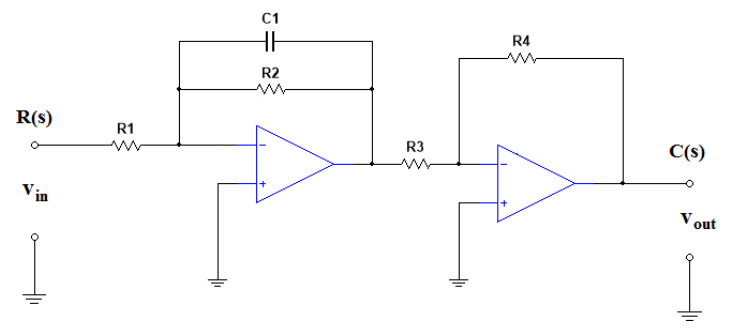
\includegraphics[width=0.5\textwidth]{../INFORME PREVIO/media/circuito-inicial}
		\caption{Sistema de primer orden con Amplificadores Operacionales}
		\label{fig:circuito-inicial}
	\end{figure}
	
	
	La función de transferencia de un circuito es la relación de la entrada con la salida de un determinado sistema en concreto para este caso se tiene un sistema de Amplificadores Operacionales de primer orden y para la obtención del comportamiento de este en función de sus parámetros, será necesario tomar como referencia un punto intermedio (salida del primer Amp. Operacional) para aislar etapas y facilitar el calculo, siendo así que en \ref{eq:ft-1} se define de forma simbólica la relación a obtener
	
	\begin{equation}
		H(s) = \frac{C(s)}{V_i(s)}
		\label{eq:ft-1}
	\end{equation}
	
	Al relacionar la señal de salida con la entrada mediante los parámetros que componen al sistema, se tiene la siguiente relación en función de sus resistencias y capacitancias la cual se describe en \ref{eq:ft}
	
	\begin{equation}
		H(s) = \frac{R_2 R_4}{R_1 R_3(1 + R_2 C_1 S)}
		\label{eq:ft}
	\end{equation}
	
	De forma general un sistema de primer orden como de define en \cite{ogata2015} estará caracterizado por la siguiente relación definida en \ref{eq:primer-orden}
	
	\begin{equation}
		H(s) = \frac{K}{1 + \tau s }
		\label{eq:primer-orden}
	\end{equation}
	
	Y en la cual se definen 2 parámetros, la ganancia $K$ y la constante de tiempo $\tau$, parámetros sobre los cuales esta condicionada la respuesta del sistema. \\
	
	En tal sentido reordenando la función de transferencia definida en \ref{eq:ft}, para asemejar tal expresión a la relación en \ref{eq:primer-orden} se tendrá la siguiente relación
	
	\begin{equation}
		H(s) = \frac{ \frac{R_2 R_4}{R_1 R_3} }{1 + R_2 C_1 S}
		\label{eq:ft-2}
	\end{equation}
	
	\section{Variando los valores de las resistencias y condensadores diseñar un circuito con el polo asignado}
	
	Como se puede observar en \ref{eq:ft-2} la ganancia $K$ estaría definida por la relación de resistencias y la constante de tiempo $\tau$ por el producto de la resistencia $R_2$ y $C_1$. \\
	
	Por otro lado para la obtención del polo deseado asignado solo será necesario igualar en el denominador el factor $\frac{1}{R_2 C_1}$, obteniendo esta expresión al factorizar la constante del tiempo de la función de transferencia definida en \ref{eq:ft-2}, es así que se tiene la siguiente expresión definida en \ref{eq:polo}
	
	\begin{equation}
		\frac{1}{R_2 C_1} = 60
		\label{eq:polo}
	\end{equation}
	
	En la ecuación \ref{eq:polo} se puede apreciar la relación entre la capacitancia y la resistencia de forma que un valor dependerá del otro en tal sentido debido a las limitantes comerciales para las capacitancias se eligió un valor para $C_1$ definiendo $R_2$ en función del polo y la capacitancia de la siguiente forma:
	
	\begin{equation}
		R_2 = \frac{1}{60 C_1}
		\label{eq:calc-resistencia}
	\end{equation}
	En función a esta nueva relación se vario el valor de la capacitancia, obteniendo distintos valores para $R_2$ los cuales se detallan en la tabla \ref{tab:resistencias}.
	
	\begin{table}[h]
		\centering
		\begin{tabular}{|c|c|}
			\hline
			\textbf{Capacitancia [uF]} & \textbf{Resistencia [$\Omega$]} \\ \hline
			1           & 16666,67             \\ \hline
			10          & 1666,67             \\ \hline
			100         & 166,67             \\ \hline
		\end{tabular}
		\caption{Valores de resistencia en función de la capacitancia}
		\label{tab:resistencias}
	\end{table}
	
	En función a los resultados antes mostrados el valor de resistencia optimo para la implementación del circuito fue 1.6K$\Omega$ valor que nos permitirá definir correctamente la polarización de los Amp. Operacionales en CD. \\\
	
	Finalmente como se busca un sistema de primer orden lo recomendable es que la ganancia $K$ sea igual a 1 por lo tanto las resistencias desde $R_1$ hasta $R_4$ tendràn el mismo valor equivalente a 1.6K$\Omega$, obteniendo un sistema de la siguiente forma con un polo ubicado en -60.
	
	\begin{equation}
		H(s) = \frac{1}{1 + 0.0167S}
		\label{eq:ft-final}
	\end{equation}
	
	Y del cual en \ref{eq:ft-final} se puede distinguir que la constante de tiempo $\tau$ será igual a 0.0167
	
	\section{Usando Matlab, simule la función de transferencia, considerando como entrada $V_in$}
	
	Para la simulación en MATLAB se hizo del diagrama de bloques y elementos eléctricos de la siguiente forma como se puede apreciar en la figura \ref{fig:circuito-matlab}
	
	\begin{figure}[h]
		\centering
		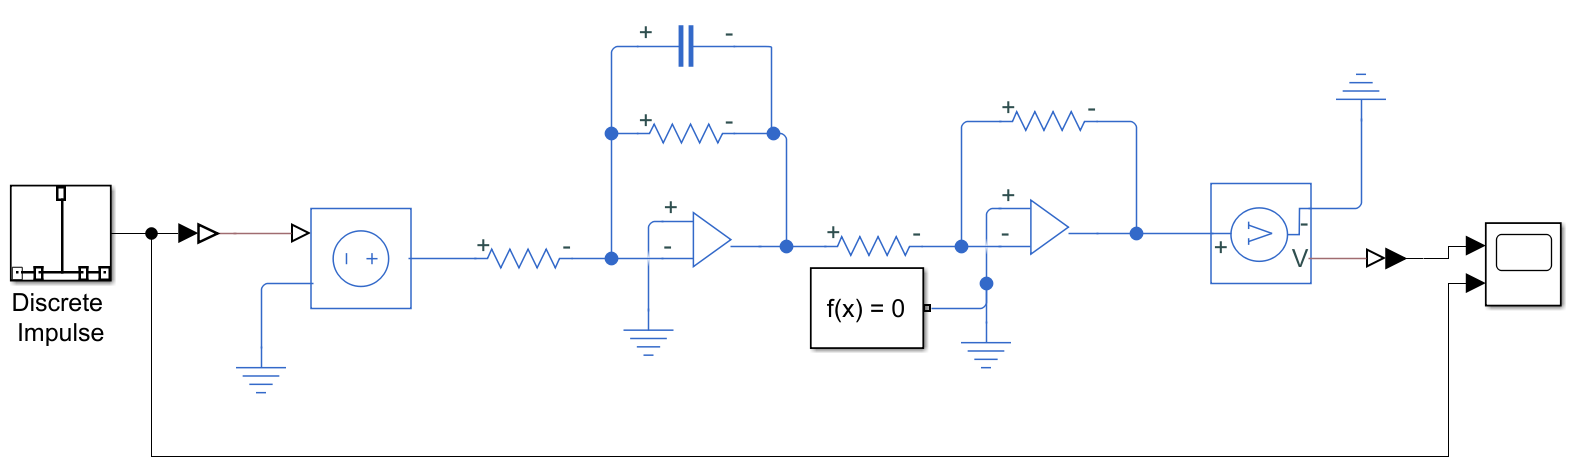
\includegraphics[width=0.5\textwidth]{../INFORME PREVIO/media/circuito-matlab}
		\caption{Circuito simulado en MATLAB}
		\label{fig:circuito-matlab}
	\end{figure}
	
	En la simulación se definieron los valores de capacitancia y resistencia previamente calculados, en la entrada se pueden definir una entrada diferente según lo requerido y la salida se mostrará mediante un osciloscopio mostrando la señal de salida con respecto a la entrada ello con la finalidad de poder comparar ambas señales.
	
	\subsection{Impulso}
	Salida frente a una entrada del tipo impulso unitario
	\begin{figure}[h]
		\centering
		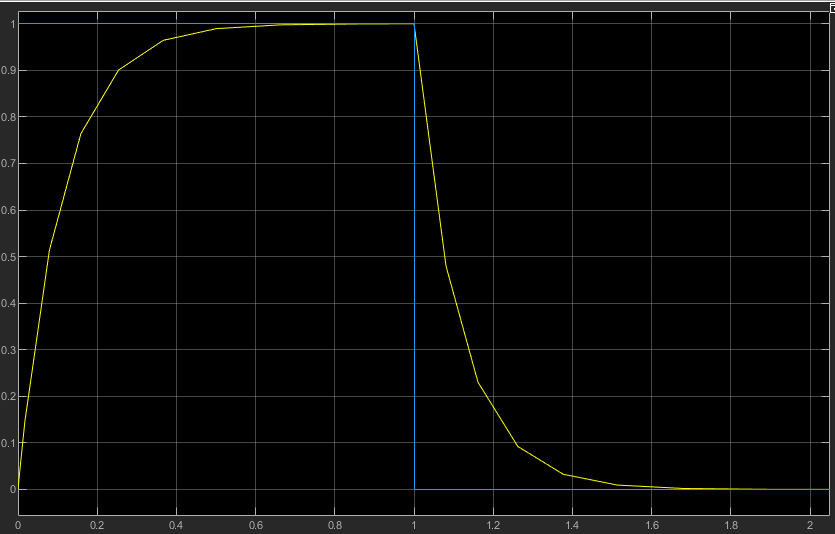
\includegraphics[width=0.4\textwidth]{../INFORME PREVIO/media/impulso}
		\caption{Respuesta frente al impulso unitario}
		\label{fig:impulso}
	\end{figure}
	
	
	\subsection{Escalón Unitario}
	Salida frente a una entrada del tipo escalón unitario
	\begin{figure}[h]
		\centering
		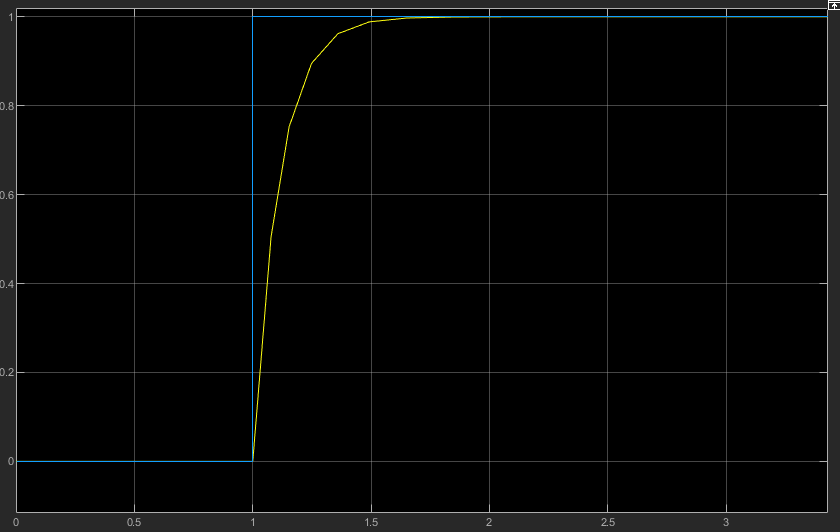
\includegraphics[width=0.4\textwidth]{../INFORME PREVIO/media/escalon_unitario}
		\caption{Respuesta frente al escalón unitario}
		\label{fig:escalonunitario}
	\end{figure}
	
	\subsection{Rampa}
	Salida frente a una entrada del tipo Rampa Unitaria
	\begin{figure}[h]
		\centering
		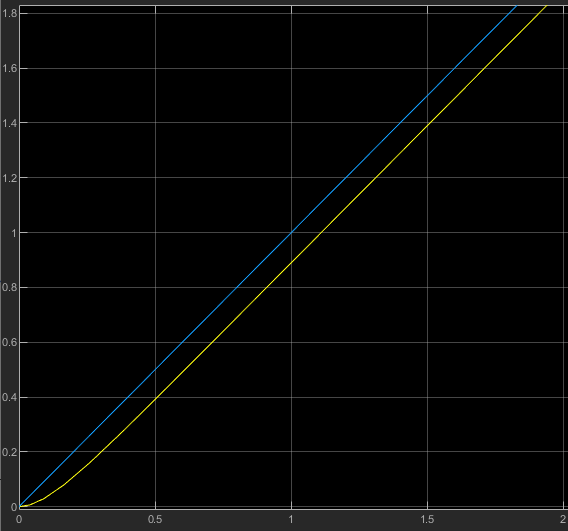
\includegraphics[width=0.4\textwidth]{../INFORME PREVIO/media/rampa}
		\caption{Respuesta frente a una entrada rampa}
		\label{fig:rampa}
	\end{figure}
	
	Para cada figura se puede apreciar que la señal de salida se representa de color amarillo, la cual nos indica que esta se aproxima o tiene un forma de tendencia a la señal de entrada con cierta variación en su respuesta a causa del sistema de forma particular a causa de la ganancia y la constante de tiempo que caracteriza al sistema.
	
	\section{Para la entrada escalón unitario}
	\subsection{Determinar la constante de tiempo}
	La constante de tiempo en relación a la ecuación \ref{eq:ft-2} será el producto de la capacitancia por la resistencia $R_2$ lo cual nos dará como resultado una constante de tiempo equivalente a 0.0167s
	
	\begin{figure}[h]
		\centering
		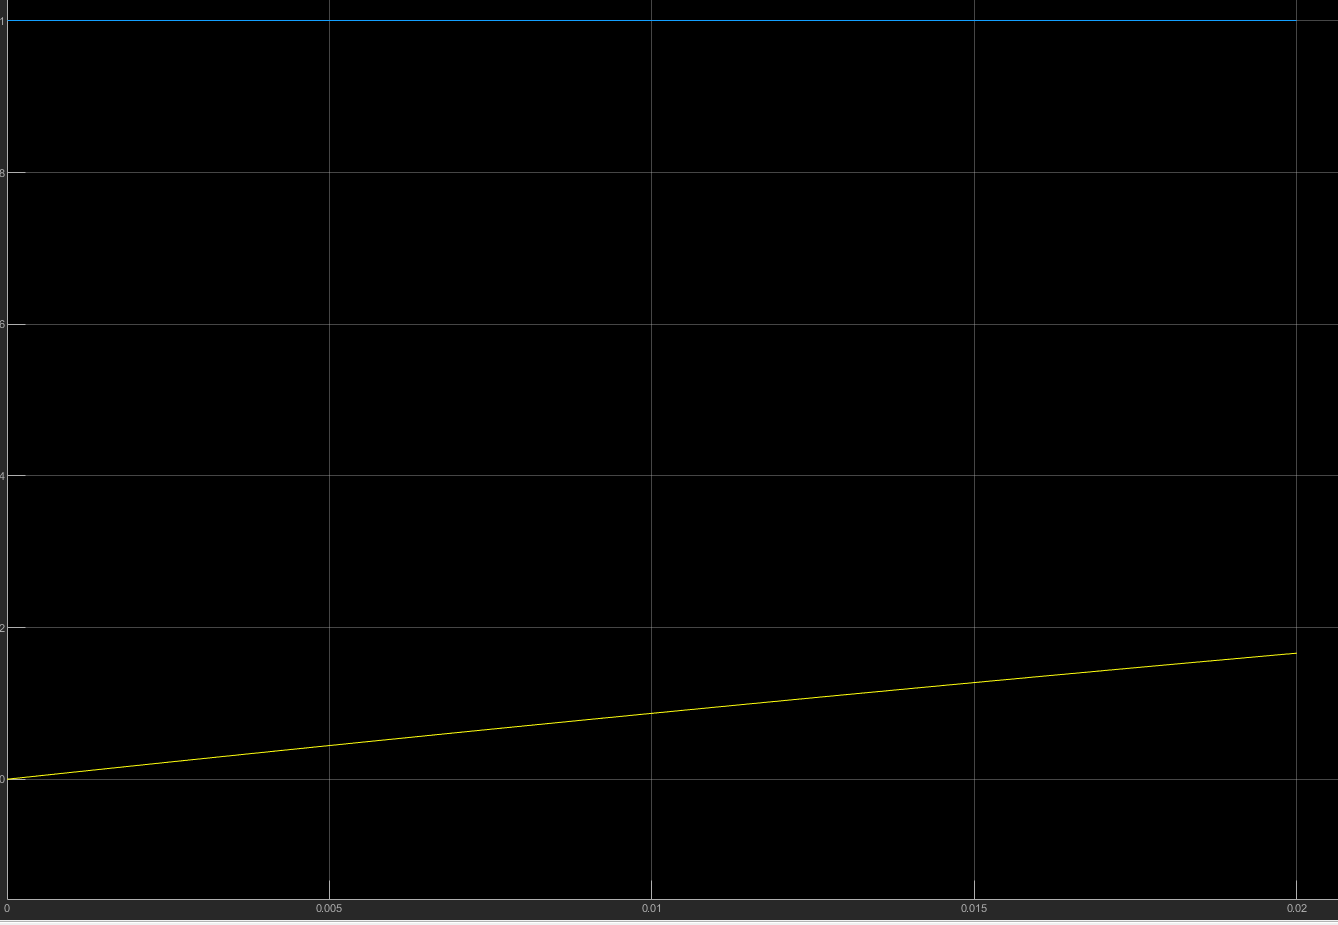
\includegraphics[width=0.5\textwidth]{../INFORME PREVIO/media/tau-escalon}
		\caption{Constante de tiempo}
		\label{fig:tau-escalon}
	\end{figure}
	
	Para la verificación de este calculo se toma como respuesta la salida del sistema en el tiempo previamente indicado para la constante de tiempo y en la  cual se puede mostrar las respuesta del circuito al 63.2 por ciento de la señal de entrada.
	
	\subsection{La pendiente de la línea tangente a la curva de respuesta en t = 0}
	Una característica relevante de los sistemas de primer orden son es que la pendiente de la respuesta del sistema es de carácter $\frac{1}{\tau}$ como se indica en siendo tal pendiente.
	
	\begin{equation}
		m = \frac{1}{0.0167} = 59.88
	\end{equation}
	
	\subsection{El valor la salida cuando t = 4T, también expréselo en porcentaje}
	
	Cuando la salida sea 4 veces la constante de tiempo la salida sera equivalente a casi el 99\%  de la señal de entrada esto se aprecia de forma directa en la gráfica de salida que se aprecia en la figura \ref{fig:escalonunitario}
	
	\section{Simulación en Multisim}
	Para simular el circuito en un entorno diferente a MATLAB se hizo uso de Multisim en el cual se definieron parámetros adicionales como la polarización de cada Amp. Operacional y para observar las salidas también se hizo uso de un osciloscopio en el cual se podrá compara la señal de salidas para las entradas senoidales, triangullar y tren de impulsos.
	
	\subsection{Señal Cuadrada}
	
	\begin{figure}[h]
		\centering
		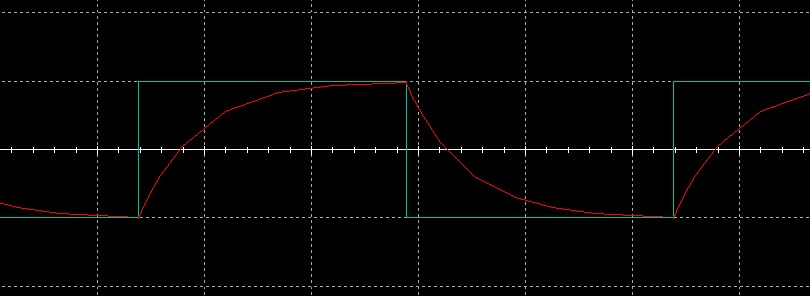
\includegraphics[width=0.5\textwidth]{../INFORME PREVIO/media/cuadrada}
		\caption{Respuesta a una señal cuadrada}
		\label{fig:cuadrada}
	\end{figure}
	
	\subsection{Señal Triangular}
	
	\begin{figure}[h]
		\centering
		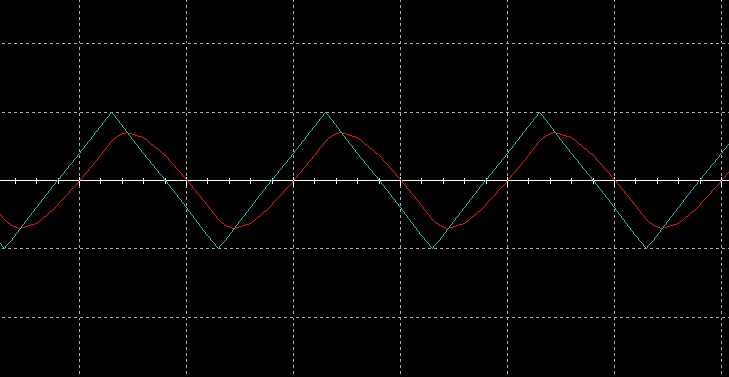
\includegraphics[width=0.5\textwidth]{../INFORME PREVIO/media/triangular}
		\caption{Respuesta a una señal triangular}
		\label{fig:triangular}
	\end{figure}
	
	\subsection{Señal Sinusoidal}
	
	\begin{figure}
		\centering
		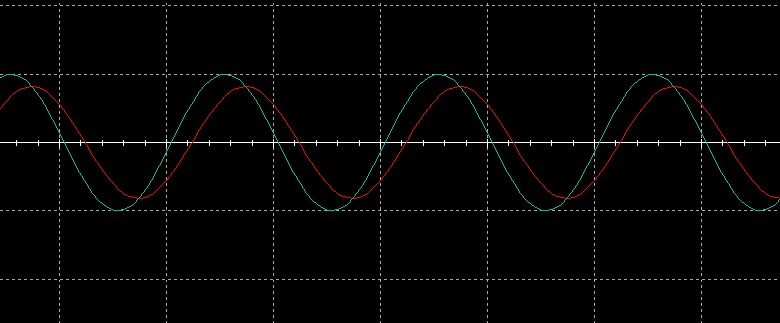
\includegraphics[width=0.5\textwidth]{../INFORME PREVIO/media/sinusoidal}
		\caption{Respuesta a una señal sinusoidal}
		\label{fig:sinusoidal}
	\end{figure}
	
	\section{Mostrar las gráficas del ítem anterior, ¿cuál es la explicación de estas gráficas?}
	Las gráficas ilustran cómo un sistema de control de primer orden responde a diferentes tipos de señales, resaltando su capacidad de seguimiento y los efectos del retardo y la suavización en comparación con las señales de entrada, además debido a la configuración del sistema, estás señales se ven atenuadas en comparación a la señal de entrada lo que permite inferir que la ganancia general será menor a la unidad.
	
	\section{Informe Final}
	Para realizar el análisis de primer orden se vio que la respuesta que brinda mayor información sobre su comportamiento, fue la señal escalón unitario la cual permite verificar el valor de la constante de tiempo, hallada teóricamente y el tiempo de establecimiento para el sistema de primer orden.
	
	\subsection{¿Cuál es la contante de tiempo del circuito diseñado?}
	Para el diseño del sistema se considero el polo $S = -9$, polo que se encontró definido por el producto de la resistencia y capacitancia del circuito de entrada y definido matemáticamente de la siguiente forma $ R_2C_1 $ y que describen el comportamiento de sistema respecto al tiempo de respuesta frente a una entrada.
	
	La constante de tiempo $\tau$ para el circuito implementado para un valor de $R_2 = 1.1K\varOmega $ y $C_1 = 100\mu F$, será: 
	\begin{equation}
		\tau = 0.11s
	\end{equation}
	\begin{figure}[h]
		\centering
		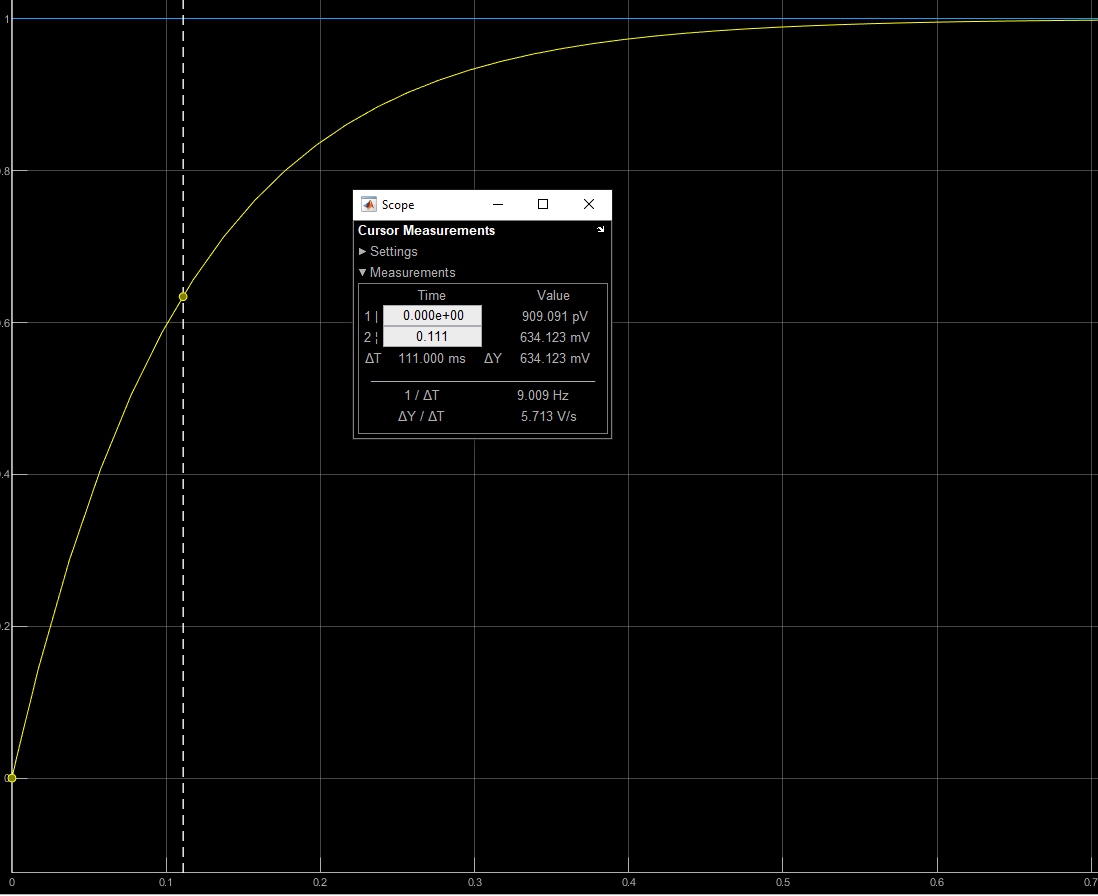
\includegraphics[width=0.4\textwidth]{media/cons_tiempo}
		\caption{Constante de tiempo frente a la entrada escalón unitario}
		\label{fig:constiempo}
	\end{figure}
	
	\subsection{¿Cuál es la pendiente de la línea de tangente a la curva de respuesta en t = 0?}
	\subsection{¿Cual es el valor de salida cuando t = 4T?}
	\section{¿La respuesta del modelo matemático hallado en forma teórica es igual o similar al circuito implementado?
	}
	\section{¿Qué se consigue al modelar teóricamente una planta?}
	
	% Bibliografía
	\bibliographystyle{IEEEtran}
	\bibliography{biblio}
	
\end{document}
